\section{Infrared anomalous dimensions}
\label{app:IRanomalousdimensions}

The on-shell method is not directly sensitive to the UV anomalous dimension associated with a certain operator $\gamma_{i\leftarrow j}$ but rather to the difference between it and the IR anomalous dimension matrix, $\delta_{ij} \gamma_{i,\text{IR}}$. 
Its knowledge is a necessary ingredient for the method, and therefore it is of paramount importance to understand how to treat it properly. 

There are two main approaches to IR divergences within the scope of the on-shell method. 
The first one consists in taking the IR anomalous dimensions to be external inputs from other computations. 
For instance, at one-loop level the IR anomalous dimension can be parametrized, in any gauge theory, as 
%
\begin{equation}
    \gamma_{\text{IR}}^{(1)} (\{p_i\}, \mu) = \frac{g^2}{4 \pi^2} \sum_{i<j} T^a_{ik} T^a_{kj} \log \frac{\mu}{-s_{ij}} + \sum_i \gamma_i^{\text{coll.}}
\end{equation}
%
where $T_{ik}^a$ are the gauge-group generators acting on the particle $i$ \cite{Becher:2009cu}. 
The first term of the IR anomalous dimension stems from soft wide-angle IR radiation, whereas the second one describes the effects arising from hard, collinear divergences. 

Alternatively, one can compute the IR anomalous dimensions via on-shell techniques by making use of the on-shell method \cite{Caron-Huot:2016cwu}.
%
Indeed,
IR divergences do not depend specifically on the gauge-invariant operator appearing within the definition of a form factor, but only on its external states. As a consequence, one can compute these quantities by simply considering a local, gauge-invariant operator with a vanishing UV anomalous dimension and allowing for two-particle interactions.
In this respect, a natural candidate is given by the energy-momentum tensor $T_{\mu\nu}$.
Since the energy-momentum tensor has to be conserved also at the quantum level, its UV anomalous dimension has to vanish, i.e.,~$\gamma_{T} = 0$, and we are left with 
\begin{equation}
\label{eq:Master_Formula_LO}
- \gamma_{\text{IR}}^{(1)} \, F_T = D \, F_T \qquad \implies \qquad \gamma_{\text{IR}}^{(1)} = -\frac{D \, F_T}{F_T} = \frac{1}{\pi} \frac{(\mathcal M F_T)^{(1)} }{F_T}\,.
\end{equation}

In this appendix, we are going to make use of the on-shell method to compute the IR collinear anomalous dimensions associated with the external particle states related to those operators we have considered within the main text.

\subsection{$\phi \bar f f$  and $\phi \bar f i  \gamma_5 f$ operators}\label{sec:IRphiffb}

The IR anomalous dimension $\gamma_{S,\text{IR}}$ associated with the operators $\phi \bar f_i f_j$  and $\phi \bar f_i i  \gamma_5 f_j$ can be
computed through the master formula
\begin{equation}
    \gamma_{S,\text{IR}} F_T^{\alpha\beta\dot\alpha\dot\beta}|_{*}(1^-_{f_i^I},2^+_{\bar f_j^J})=\frac{1}{\pi}(\mathcal M F_T^{\alpha\beta\dot\alpha\dot\beta})|_{*}(1^-_{f_i^I},2^+_{\bar f_j^J})\,,
\end{equation}
which diagrammatically reads as in Fig.~\ref{fig:phiffIR}.

\begin{figure}[htbp]
\centering
\includegraphics[width=\textwidth,page=13]{figures/diagrams.pdf}
\caption{Diagrammatic formula for computing $\gamma_{S,\text{IR}}$.}
\label{fig:phiffIR}
\end{figure}

On the left-hand side, we have the form factor of the fermion stress-energy tensor
\begin{equation}
    F_T^{\alpha\beta\dot\alpha\dot\beta}|_{*}(1_{f_i^I}^{-},2_{\bar f_j^J}^{+}) = \delta^{ij}\delta_{IJ}\mathcal T^{\alpha\beta\dot\alpha\dot\beta}_{12}
\end{equation}
where we have defined
\begin{equation}
    \mathcal T^{\alpha\beta\dot\alpha\dot\beta}_{12} = \frac{1}{2}\left( \lambda_1^\alpha \lambda_1^\beta \tilde\lambda_1^{\dot\alpha} \tilde\lambda_2^{\dot\beta} + \lambda_1^\alpha \lambda_1^\beta \tilde\lambda_2^{\dot\alpha} \tilde\lambda_1^{\dot\beta} - \lambda_1^\alpha \lambda_2^\beta \tilde\lambda_2^{\dot\alpha} \tilde\lambda_2^{\dot\beta} - \lambda_2^\alpha \lambda_1^\beta \tilde\lambda_2^{\dot\alpha} \tilde\lambda_2^{\dot\beta}  \right)\,,
\end{equation}
while, on the right-hand side, the convolution is expanded allowing for all possible intermediate states
\begin{align}
    (\mathcal M F_T^{\alpha\beta\dot\alpha\dot\beta})|_{*}(1_{f_i^I}^{-},2_{\bar f_j^J}^{+}) &= \sum_{h_1,h_2}\int d\text{LIPS}_2\,
    \bigg[\sum_{f'}
     \mathcal M|_{*} (1_{f_i^I}^{-},2_{\bar f_j^J}^{+}; x_{f_k'^K}^{h_1},y_{\bar f_l'^L}^{h_2})F_T^{\alpha\beta\dot\alpha\dot\beta}|_{*}(x_{f_k'^K}^{h_1},y_{\bar f_l'^L}^{h_2})\nonumber \\
    &\quad + \mathcal M|_{*} (1_{f_i^I}^{-},2_{\bar f_j^J}^{+}; x_\gamma^{h_1},y_\gamma^{h_2})F_T^{\alpha\beta\dot\alpha\dot\beta}|_{*}(x_\gamma^{h_1},y_\gamma^{h_2})\nonumber \\
    &\quad+ \mathcal M|_{*} (1_{f_i^I}^{-},2_{\bar f_j^J}^{+}; x_{g^c}^{h_1},y_{g^d}^{h_2})F_T^{\alpha\beta\dot\alpha\dot\beta}|_{*}(x_{g^c}^{h_1},y_{g^d}^{h_2})
    \bigg]\,.
\end{align}
The amplitudes that give a non-vanishing contribution are
\begin{align}
    \mathcal M|_{*} (1_{f_i^I}^{-},2_{\bar f_j^J}^{+}; x_{f_k'^K}^{-},y_{\bar f_l'^L}^{+})\delta_{KL} &= 
    -2\delta_{IJ}\bigg[\frac{e^2Q_f^2+C_Fg_s^2c_f^2}{\agl{1}{x}\sqr{x}{1}}\delta_{ff'}\delta^{ik}\delta^{jl} + N_{f'}\frac{e^2Q_f Q_{f'}}{\agl{1}{2}\sqr{2}{1}} \delta^{ij}\delta^{kl}\bigg]\nonumber \\&\quad\times \agl{1}{y}\sqr{x}{2}
    \,, \\
    \mathcal M|_{*} (1_{f_i^I}^{-},2_{\bar f_j^J}^{+}; x_{f_k'^K}^{+},y_{\bar f_l'^L}^{-})\delta_{KL} &= 
    -2\delta_{IJ} N_{f'}e^2Q_f Q_{f'}\delta^{ij}\delta^{kl} \frac{ \agl{1}{x}\sqr{y}{2}}{\agl{1}{2}\sqr{2}{1}}\,,  \\
    \mathcal M|_*(1^-_{f_i^I},2^+_{\bar f_j^J};x^-_\gamma,y^+_\gamma) &= -2e^2Q_f^2\delta^{ij}\delta_{IJ}\frac{\agl{1}{y}\sqr{x}{2}}{\agl{1}{x}\sqr{y}{1}}\,, \\
    \mathcal M|_*(1^-_{f_i^I},2^+_{\bar f_j^J};x^+_\gamma,y^-_\gamma) &= -2e^2Q_f^2\delta^{ij}\delta_{IJ}\frac{\agl{1}{x}\sqr{y}{2}}{\agl{1}{y}\sqr{x}{1}}\,,\\
    \mathcal M|_*(1^-_{f_i^I},2^+_{\bar f_j^J};x^-_{g^a},y^+_{g^b})\delta^{ab} &= -2C_Fg_s^2c_f^2\delta^{ij}\delta_{IJ}\frac{\agl{1}{y}\sqr{x}{2}}{\agl{1}{x}\sqr{y}{1}}\,, \\
    \mathcal M|_*(1^-_{f_i^I},2^+_{\bar f_j^J};x^+_{g^a},y^-_{g^b})\delta^{ab} &= -2C_Fg_s^2c_f^2\delta^{ij}\delta_{IJ}\frac{\agl{1}{x}\sqr{y}{2}}{\agl{1}{y}\sqr{x}{1}}\,,
\end{align}
(where $N_{f'}=c_{f'}N_c + (1 - c_{f'})$, namely $N_{f'}=N_c$ if $f'=q$ and $N_{f'}=1$ if $f'=\ell$) which are respectively multiplied by
\begin{align}
    F_T^{\alpha\beta\dot\alpha\dot\beta}|_{*}(x_{f_k'^K}^{-},y_{\bar f_l'^L}^{+}) &= \delta^{kl}\delta_{KL}\mathcal T^{\alpha\beta\dot\alpha\dot\beta}_{xy} \,,&
    F_T^{\alpha\beta\dot\alpha\dot\beta}|_{*}(x_{f_k'^K}^{+},y_{\bar f_l'^L}^{-}) &= -\delta^{kl}\delta_{KL}\mathcal T^{\alpha\beta\dot\alpha\dot\beta}_{yx}\,,\\
    F_T^{\alpha\beta\dot\alpha\dot\beta}|_{*}(x_{\gamma}^{-},y_{\gamma}^{+}) &= -2\lambda_x^\alpha \lambda_x^\beta \tilde\lambda_y^{\dot\alpha} \tilde\lambda_y^{\dot\beta}\,, &
    F_T^{\alpha\beta\dot\alpha\dot\beta}|_{*}(x_{\gamma}^{+},y_{\gamma}^{-}) &= -2\lambda_y^\alpha \lambda_y^\beta \tilde\lambda_x^{\dot\alpha} \tilde\lambda_x^{\dot\beta}\,, \\
    F_T^{\alpha\beta\dot\alpha\dot\beta}|_{*}(x_{g^a}^{-},y_{g^b}^{+}) &= -2\delta^{ab}\lambda_x^\alpha \lambda_x^\beta \tilde\lambda_y^{\dot\alpha} \tilde\lambda_y^{\dot\beta}\,, &
    F_T^{\alpha\beta\dot\alpha\dot\beta}|_{*}(x_{g^a}^{+},y_{g^b}^{-}) &= -2\delta^{ab}\lambda_y^\alpha \lambda_y^\beta \tilde\lambda_x^{\dot\alpha} \tilde\lambda_x^{\dot\beta}
    \,.
\end{align}

\subparagraph{Angular integration.}
The calculation of the phase-space integral with the angular parameterization is as follows.
The amplitudes read
\begin{align}
    \mathcal M|_{*} (1_{f_i^I}^{-},2_{\bar f_j^J}^{+}; x_{f_k'^K}^{-},y_{\bar f_l'^L}^{+})\delta_{KL} &= 
    2\delta_{IJ}\bigg[(e^2Q_f^2+C_Fg_s^2c_f^2)\delta_{ff'}\delta^{ik}\delta^{jl}\frac{\cos^2\theta}{\sin^2\theta}\nonumber\\ &\quad + N_{f'} e^2Q_f Q_{f'} \delta^{ij}\delta^{kl}\cos^2\theta \bigg]\,, \\
    \mathcal M|_{*} (1_{f_i^I}^{-},2_{\bar f_j^J}^{+}; x_{f_k'^K}^{+},y_{\bar f_l'^L}^{-})\delta_{KL} &= -2\delta_{IJ} N_{f'} e^2Q_f Q_{f'}\delta^{ij}\delta^{kl} \sin^2\theta e^{2i\phi}\,, \\
    \mathcal M|_*(1^-_{f_i^I},2^+_{\bar f_j^J};x^-_\gamma,y^+_\gamma) &= -2e^2Q_f^2\delta^{ij}\delta_{IJ}\frac{\cos\theta}{\sin\theta}e^{-i\phi}\,, \\
    \mathcal M|_*(1^-_{f_i^I},2^+_{\bar f_j^J};x^+_\gamma,y^-_\gamma) &= 2e^2Q_f^2\delta^{ij}\delta_{IJ}\frac{\sin\theta}{\cos\theta}e^{3i\phi}\,, \\
    \mathcal M|_*(1^-_{f_i^I},2^+_{\bar f_j^J};x^-_{g^a},y^+_{g^b})\delta^{ab} &= -2C_Fg_s^2c_f^2\delta^{ij}\delta_{IJ}\frac{\cos\theta}{\sin\theta}e^{-i\phi}\,, \\
    \mathcal M|_*(1^-_{f_i^I},2^+_{\bar f_j^J};x^+_{g^a},y^-_{g^b})\delta^{ab} &= 2C_Fg_s^2c_f^2\delta^{ij}\delta_{IJ}\frac{\sin\theta}{\cos\theta}e^{3i\phi}\,,
\end{align}
and the integration in the azimuthal angle $\phi$ yields
\begin{align}
    \int_0^{2\pi}\frac{d\phi}{2\pi}\,F_T^{\alpha\beta\dot\alpha\dot\beta}|_{*}(x_{f_k'^K}^{-},y_{\bar f_l'^L}^{+}) &= \cos^2\theta[-1+2\cos(2\theta)]\delta^{kl}\delta_{KL}\mathcal T^{\alpha\beta\dot\alpha\dot\beta}_{12}\,,\\
    \int_0^{2\pi}\frac{d\phi}{2\pi}\,F_T^{\alpha\beta\dot\alpha\dot\beta}|_{*}(x_{f_k'^K}^{+},y_{\bar f_l'^L}^{-})e^{2i\phi} &= -\sin^2\theta [1+2\cos(2\theta)]\delta^{kl}\delta_{KL}\mathcal T^{\alpha\beta\dot\alpha\dot\beta}_{12}\,, \\
    \int_0^{2\pi}\frac{d\phi}{2\pi}\,F_T^{\alpha\beta\dot\alpha\dot\beta}|_{*}(x_{\gamma}^{-},y_{\gamma}^{+})e^{-i\phi} &= -4\cos^3\theta\sin\theta \mathcal T^{\alpha\beta\dot\alpha\dot\beta}_{12}\,, \\
    \int_0^{2\pi}\frac{d\phi}{2\pi}\,F_T^{\alpha\beta\dot\alpha\dot\beta}|_{*}(x_{\gamma}^{+},y_{\gamma}^{-})e^{3i\phi} &= 4\cos\theta\sin^3\theta \mathcal T^{\alpha\beta\dot\alpha\dot\beta}_{12}\,,\\
    \int_0^{2\pi}\frac{d\phi}{2\pi}\,F_T^{\alpha\beta\dot\alpha\dot\beta}|_{*}(x_{g^a}^{-},y_{g^b}^{+})e^{-i\phi} &= -4\delta^{ab}\cos^3\theta\sin\theta \mathcal T^{\alpha\beta\dot\alpha\dot\beta}_{12}\,, \\
    \int_0^{2\pi}\frac{d\phi}{2\pi}\,F_T^{\alpha\beta\dot\alpha\dot\beta}|_{*}(x_{g^a}^{+},y_{g^b}^{-})e^{3i\phi} &= 4\delta^{ab}\cos\theta\sin^3\theta \mathcal T^{\alpha\beta\dot\alpha\dot\beta}_{12}\,.
\end{align}
Therefore, the remaining integral to compute is
\begin{align}
    (\mathcal M F_T^{\alpha\beta\dot\alpha\dot\beta})|_{*}(1^-_{f_i^I},2^+_{\bar f_j^J}) &= \frac{1}{16\pi}\int_0^{\pi/2}2\sin\theta\cos\theta \,d\theta\,\bigg[2\sum_{f'}2 N_{f'}e^2Q_f Q_{f'}\sin^4\theta [1+2\cos(2\theta)]\nonumber \\
    &\quad +2\sum_{f'}2 N_{f'}e^2Q_f Q_{f'}\cos^4\theta[-1+2\cos(2\theta)]\nonumber \\
    &\quad +4(e^2Q_f^2+C_Fg_s^2c_f^2)\frac{\cos^4\theta}{\sin^2\theta}[-1+2\cos(2\theta)]\nonumber \\
    &\quad  +8(e^2Q_f^2+C_Fg_s^2c_f^2)(\cos^4\theta + \sin^4\theta)
    \bigg]F_T^{\alpha\beta\dot\alpha\dot\beta}|_{*}(1^-_{f_i^I},2^+_{\bar f_j^J})\nonumber \\
    &= \frac{1}{4\pi}(e^2Q_f^2+C_Fg_s^2c_f^2)\int_0^{\pi/2}2\sin\theta\cos\theta \,d\theta\,\bigg[\frac{\cos^4\theta}{\sin^2\theta}[-1+2\cos(2\theta)]\nonumber\\
    &\quad +2(\cos^4\theta + \sin^4\theta) \bigg]
    F_T^{\alpha\beta\dot\alpha\dot\beta}|_{*}(1^-_{f_i^I},2^+_{\bar f_j^J})\,,
\end{align}
which implies
\begin{equation}\label{eq:gammaS_IR_angular}
    \gamma_{S,\text{IR}} = \frac{1}{4\pi^2}(e^2Q_f^2+C_Fg_s^2c_f^2)\int_0^{\pi/2}2\sin\theta\cos\theta \,d\theta\,\bigg[\frac{\cos^4\theta}{\sin^2\theta}[-1+2\cos(2\theta)]+2(\cos^4\theta + \sin^4\theta) \bigg]\,.
\end{equation}

\subparagraph{Stokes integration.}
The calculation of the phase-space integral with the Stokes parameterization is as follows.
The amplitudes read
\begin{align}
%m1
    \mathcal M|_{*} (1_{f_i^I}^{-},2_{\bar f_j^J}^{+}; x_{f_k'^K}^{-},y_{\bar f_l'^L}^{+})\delta_{KL} &= 
2\delta_{IJ}\bigg[(e^2Q_f^2+C_Fg_s^2c_f^2)\delta_{ff'}\delta^{ik}\delta^{jl}\frac{1}{z \zb}\nonumber\\ &\quad + N_{f'} e^2Q_f Q_{f'} \delta^{ij}\delta^{kl}\frac{1}{1+z\zb} \bigg]\,, \\
%m2
    \mathcal M|_{*} (1_{f_i^I}^{-},2_{\bar f_j^J}^{+}; x_{f_k'^K}^{+},y_{\bar f_l'^L}^{-})\delta_{KL} &= -2\delta_{IJ} N_{f'} e^2Q_f Q_{f'}\delta^{ij}\delta^{kl}\frac{\zb^2}{1+z\zb}\,, \\
%m3
    \mathcal M|_*(1^-_{f_i^I},2^+_{\bar f_j^J};x^-_\gamma,y^+_\gamma) &= 2e^2Q_f^2\delta^{ij}\delta_{IJ}\frac{1}{\zb}\,, \\
%m4
    \mathcal M|_*(1^-_{f_i^I},2^+_{\bar f_j^J};x^+_\gamma,y^-_\gamma) &= -2e^2Q_f^2\delta^{ij}\delta_{IJ}\frac{\zb^2}{z}\,, \\
%m5
    \mathcal M|_*(1^-_{f_i^I},2^+_{\bar f_j^J};x^-_{g^a},y^+_{g^b})\delta^{ab} &= 2C_Fg_s^2c_f^2\delta^{ij}\delta_{IJ}\frac{1}{\zb}\,, \\
%m6
    \mathcal M|_*(1^-_{f_i^I},2^+_{\bar f_j^J};x^+_{g^a},y^-_{g^b})\delta^{ab} &= -2C_Fg_s^2c_f^2\delta^{ij}\delta_{IJ}\frac{\zb^2}{z}\,,
\end{align}
which lead to
\begin{equation}
    (\mathcal M F_T^{\alpha\beta\dot\alpha\dot\beta})|_{*}(1^-_{f_i^I},2^+_{\bar f_j^J}) =  -\frac{3}{8\pi}(e^2Q_f^2+C_Fg_s^2c_f^2) \ F_T^{\alpha\beta\dot\alpha\dot\beta}|_{*}(1^-_{f_i^I},2^+_{\bar f_j^J})
\end{equation}
and thus
\begin{equation}\label{eq:gammaS_IR_stokes}
    \gamma_{S,\text{IR}} = -\frac{3}{8\pi^2}(e^2Q_f^2+C_Fg_s^2c_f^2)\,.
\end{equation}

\subsection{$\phi FF$  and $\phi F\tilde F$ operators}\label{sec:IRphigammagamma}

The IR anomalous dimension $\gamma_{\gamma,\text{IR}}$ associated with the operators $\phi FF$  and $\phi F\tilde F$ can be computed through the master formula
\begin{equation}
    \gamma_{\gamma,\text{IR}} F_T^{\alpha\beta\dot\alpha\dot\beta}|_{*}(1^-_\gamma,2^+_\gamma)=\frac{1}{\pi}(\mathcal M F_T^{\alpha\beta\dot\alpha\dot\beta})|_{*}(1^-_\gamma,2^+_\gamma)\,,
\end{equation}
which diagrammatically reads as in Fig.~\ref{fig:phigammagammaIR}.

\begin{figure}[htbp]
\centering
\includegraphics[width=\textwidth,page=11]{figures/diagrams.pdf}
\caption{Diagrammatic formula for computing $\gamma_{\gamma,\text{IR}}$.}
\label{fig:phigammagammaIR}
\end{figure}

On the left-hand side, we have the form factor of the photon stress-energy tensor 
\begin{equation}
    F_T^{\alpha\beta\dot\alpha\dot\beta}|_{*}(1^-_\gamma,2^+_\gamma) = -2 \lambda_1^\alpha \lambda_1^\beta \tilde\lambda_2^{\dot\alpha} \tilde\lambda_2^{\dot\beta}\,,
\end{equation}
while, on the right-hand side, the convolution is expanded allowing for all possible intermediate states
\begin{align}
    (\mathcal M F_T^{\alpha\beta\dot\alpha\dot\beta})|_{*}(1^-_\gamma,2^+_\gamma) &= \sum_{h_1,h_2}\int d\text{LIPS}_2\,
    \bigg[
    \sum_f  \mathcal M|_{*} (1^-_\gamma,2^+_\gamma; x_{f_i}^{h_1},y_{\bar f_j}^{h_2})F_T^{\alpha\beta\dot\alpha\dot\beta}|_{*}(x_{f_i}^{h_1},y_{\bar f_j}^{h_2})\nonumber \\
    &\quad + \mathcal M|_{*} (1^-_\gamma,2^+_\gamma; x_\gamma^{h_1},y_\gamma^{h_2})F_T^{\alpha\beta\dot\alpha\dot\beta}|_{*}(x_\gamma^{h_1},y_\gamma^{h_2})\nonumber \\
    &\quad + \mathcal M|_{*} (1^-_\gamma,2^+_\gamma; x_{g^a}^{h_1},y_{g^b}^{h_2})F_T^{\alpha\beta\dot\alpha\dot\beta}|_{*}(x_{g^a}^{h_1},y_{g^b}^{h_2})
    \bigg]\,.
\end{align}
The only nonvanishing amplitudes are
\begin{align}
    \mathcal M|_{*} (1^-_\gamma,2^+_\gamma; x_{f_i}^{-},y_{\bar f_j}^{+}) &= 2e^2 Q_f^2 \delta^{ij}\frac{\agl{1}{y}\sqr{2}{x}}{\agl{2}{y}\sqr{1}{y}}\,, \\
    \mathcal M|_{*} (1^-_\gamma,2^+_\gamma; x_{f_i}^{+},y_{\bar f_j}^{-}) &= 2e^2 Q_f^2 \delta^{ij}\frac{\agl{1}{x}\sqr{2}{y}}{\agl{2}{y}\sqr{1}{y}}\,,
\end{align}
which are respectively multiplied by
\begin{align}
F_T^{\alpha\beta\dot\alpha\dot\beta}|_{*}(x_{f_i}^{-},y_{\bar f_j}^{+}) = \delta^{ij}\mathcal{T}_{xy}^{\alpha\beta\dot{\alpha}\dot{\beta}}\,, \qquad 
F_T^{\alpha\beta\dot\alpha\dot\beta}|_{*}(x_{f_i}^{+},y_{\bar f_j}^{-}) = -\delta^{ij}\mathcal{T}_{yx}^{\alpha\beta\dot{\alpha}\dot{\beta}}\,.
\end{align}

\subparagraph{Angular integration.}
The calculation of the phase-space integral with the angular parameterization is as follows.
The amplitudes read
\begin{align}
    \mathcal M|_{*} (1^-_\gamma,2^+_\gamma; x_{f_i}^{-},y_{\bar f_j}^{+}) &= 2e^2 Q_f^2 \delta^{ij}\frac{\cos\theta}{\sin\theta}e^{i\phi}\,, \\
    \mathcal M|_{*} (1^-_\gamma,2^+_\gamma; x_{f_i}^{+},y_{\bar f_j}^{-}) &= -2e^2 Q_f^2 \delta^{ij}\frac{\sin\theta}{\cos\theta}e^{3i\phi}\,,
\end{align}
and the integration in the azimuthal angle $\phi$ yields
\begin{align}
    \int_0^{2\pi}\frac{d\phi}{2\pi}\,F_T^{\alpha\beta\dot\alpha\dot\beta}|_{*}(x_{f_i}^{-},y_{\bar f_j}^{+})e^{i\phi} &= -2\delta^{ij}\lambda_1^\alpha \lambda_1^\beta \tilde\lambda_2^{\dot\alpha} \tilde\lambda_2^{\dot\beta} \cos^3\theta\sin\theta\,,  \\
    \int_0^{2\pi}\frac{d\phi}{2\pi}\,F_T^{\alpha\beta\dot\alpha\dot\beta}|_{*}(x_{f_i}^{+},y_{\bar f_j}^{-})e^{3i\phi} &=2\delta^{ij}\lambda_1^\alpha \lambda_1^\beta \tilde\lambda_2^{\dot\alpha} \tilde\lambda_2^{\dot\beta} \cos\theta\sin^3\theta \,.
\end{align}
Therefore, the remaining integral to compute is
\begin{align}
    (\mathcal M F_T^{\alpha\beta\dot\alpha\dot\beta})|_{*}(1^-_\gamma,2^+_\gamma) &= -4e^2 \lambda_1^\alpha \lambda_1^\beta \tilde\lambda_2^{\dot\alpha} \tilde\lambda_2^{\dot\beta}\frac{1}{8\pi}\int_0^{\pi/2}2\sin\theta\cos\theta \,d\theta\, (\cos^4\theta+\sin^4\theta)\sum_fQ_f^2 \nonumber \\
    &= -2\lambda_1^\alpha \lambda_1^\beta \tilde\lambda_2^{\dot\alpha} \tilde\lambda_2^{\dot\beta}\frac{e^2}{6\pi}\sum_fQ_f^2\,,
\end{align}
which implies
\begin{equation}\label{eq:gammaIRphoton}
    \gamma_{\gamma,\text{IR}} = \frac{e^2}{6\pi^2} \sum_f Q_f^2\,.
\end{equation}

\subparagraph{Stokes integration.}
By exploiting the Stokes parameterization, the amplitudes read
\begin{align}
    \mathcal M|_{*} (1^-_\gamma,2^+_\gamma; x_{f_i}^{-},y_{\bar f_j}^{+}) &= -2e^2 Q_f^2 \delta^{ij}\frac{1}{z}\,, \\
    \mathcal M|_{*} (1^-_\gamma,2^+_\gamma; x_{f_i}^{+},y_{\bar f_j}^{-}) &= 2e^2 Q_f^2 \delta^{ij}\frac{\zb^2}{z}\,,
\end{align}
and plugging everything together we obtain
\begin{align}
    (\mathcal M F_T^{\alpha\beta\dot\alpha\dot\beta})|_{*}(1^-_\gamma,2^+_\gamma) 
    &= -2\lambda_1^\alpha \lambda_1^\beta \tilde\lambda_2^{\dot\alpha} \tilde\lambda_2^{\dot\beta}\frac{e^2}{6\pi}\sum_fQ_f^2\,,
\end{align}
which implies Eq.~\eqref{eq:gammaIRphoton}.

\subsection{$\phi GG$  and $\phi G\tilde G$ operators}\label{sec:IRphigg}

The IR anomalous dimension $\gamma_{g,\text{IR}}$ associated with the operators $\phi GG$  and $\phi G\tilde G$ can be computed through the master formula
\begin{equation}
    \gamma_{g,\text{IR}} F_T^{\alpha\beta\dot\alpha\dot\beta}|_{*}(1^-_{g^a},2^+_{g^b})=\frac{1}{\pi}(\mathcal M F_T^{\alpha\beta\dot\alpha\dot\beta})|_{*}(1^-_{g^a},2^+_{g^b})
\end{equation}
which diagrammatically reads as in Fig.~\ref{fig:phigluongluonIR}.

\begin{figure}[htbp]
\centering
\includegraphics[width=\textwidth,page=12]{figures/diagrams.pdf}
\caption{Diagrammatic formula for computing $\gamma_{g,\text{IR}}$.}
\label{fig:phigluongluonIR}
\end{figure}

On the left-hand side, we have the form factor of the gluon stress-energy tensor 
\begin{equation}
    F_T^{\alpha\beta\dot\alpha\dot\beta}|_{*}(1^-_{g^a},2^+_{g^b}) = -2 \delta^{ab} \lambda_1^\alpha \lambda_1^\beta \tilde\lambda_2^{\dot\alpha} \tilde\lambda_2^{\dot\beta}\,,
\end{equation}
while, on the right-hand side, the convolution is expanded allowing for all possible intermediate states
\begin{align}
    (\mathcal M F_T^{\alpha\beta\dot\alpha\dot\beta})|_{*}(1^-_{g^a},2^+_{g^b}) &= \sum_{h_1,h_2}\int d\text{LIPS}_2\,
    \bigg[
    \sum_f  \mathcal M|_{*} (1^-_{g^a},2^+_{g^b}; x_{f_i^I}^{h_1},y_{\bar f_j^J}^{h_2})F_T^{\alpha\beta\dot\alpha\dot\beta}|_{*}(x_{f_i^I}^{h_1},y_{\bar f_j^J}^{h_2})\nonumber \\
    &\quad + \mathcal M|_{*} (1^-_{g^a},2^+_{g^b}; x_\gamma^{h_1},y_\gamma^{h_2})F_T^{\alpha\beta\dot\alpha\dot\beta}|_{*}(x_\gamma^{h_1},y_\gamma^{h_2})\nonumber \\
    &\quad + \mathcal M|_{*} (1^-_{g^a},2^+_{g^b}; x_{g^c}^{h_1},y_{g^d}^{h_2})F_T^{\alpha\beta\dot\alpha\dot\beta}|_{*}(x_{g^c}^{h_1},y_{g^d}^{h_2})
    \bigg]\,.
\end{align}
The amplitudes that give a nonvanishing contribution are
\begin{align}
    \mathcal M|_*(1^-_{g^a},2^+_{g^b};x_{f_i^I}^{-},y_{\bar f_j^J}^{+})\delta_{IJ} &= 2T_Fg_s^2c_f^2\delta^{ij}\delta^{ab}\frac{\agl{1}{y}\sqr{x}{2}}{\agl{2}{y}\sqr{y}{1}}\,, \\
    \mathcal M|_*(1^-_{g^a},2^+_{g^b};x_{f_i^I}^{+},y_{\bar f_j^J}^{-})\delta_{IJ} &= 2T_Fg_s^2c_f^2\delta^{ij}\delta^{ab}\frac{\agl{1}{x}\sqr{y}{2}}{\agl{2}{y}\sqr{y}{1}}\,,\\
    \mathcal M|_* (1^-_{g^a},2^+_{g^b};x_{g^c}^{-},y_{g^d}^{+}) \delta^{cd} &= -2C_A g_s^2\delta^{ab}\frac{\agl{1}{y}^4}{\agl{1}{x}\agl{x}{2}\agl{2}{y}\agl{y}{1}}\,, \\
    \mathcal M|_* (1^-_{g^a},2^+_{g^b};x_{g^c}^{+},y_{g^d}^{-}) \delta^{cd} &= -2C_A g_s^2\delta^{ab}\frac{\agl{1}{x}^4}{\agl{1}{x}\agl{x}{2}\agl{2}{y}\agl{y}{1}}\,,
\end{align}
which are respectively multiplied by
\begin{align}
& 
F_T^{\alpha\beta\dot\alpha\dot\beta}|_{*}(x_{f_i^I}^{-},y_{\bar f_j^J}^{+}) = \delta^{ij}\delta_{IJ}\mathcal{T}_{xy}^{\alpha\beta\dot{\alpha}\dot{\beta}}\,, 
\qquad & &
F_T^{\alpha\beta\dot\alpha\dot\beta}|_{*}(x_{f_i^I}^{+},y_{\bar f_j^J}^{-}) = -\delta^{ij}\delta_{IJ}\mathcal{T}_{yx}^{\alpha\beta\dot{\alpha}\dot{\beta}}\,, 
\\ 
&
F_T^{\alpha\beta\dot\alpha\dot\beta}|_{*}(x_{g^c}^{-},y_{g^d}^{+}) = -2\delta^{cd}\lambda_x^\alpha \lambda_x^\beta \tilde\lambda_y^{\dot\alpha} \tilde\lambda_y^{\dot\beta}\,, 
& & F_T^{\alpha\beta\dot\alpha\dot\beta}|_{*}(x_{g^c}^{+},y_{g^d}^{-}) = -2\delta^{cd}\lambda_y^\alpha \lambda_y^\beta \tilde\lambda_x^{\dot\alpha} \tilde\lambda_x^{\dot\beta}\,.
\end{align}

\subparagraph{Angular integration.}
The calculation of the phase-space integral with the angular parameterization is as follows.
The amplitudes read
\begin{align}
    \mathcal M|_*(1^-_{g^a},2^+_{g^b};x_{f_i^I}^{-},y_{\bar f_j^J}^{+})\delta_{IJ} &= 2T_Fg_s^2c_f^2\delta^{ij}\delta^{ab}\frac{\cos\theta}{\sin\theta}e^{i\phi}\,, \\
    \mathcal M|_*(1^-_{g^a},2^+_{g^b};x_{f_i^I}^{+},y_{\bar f_j^J}^{-})\delta_{IJ} &= -2T_Fg_s^2c_f^2\delta^{ij}\delta^{ab}\frac{\sin\theta}{\cos\theta}e^{3i\phi}\,,\\
    \mathcal M|_* (1^-_{g^a},2^+_{g^b};x_{g^c}^{-},y_{g^d}^{+}) \delta^{cd} &= 2C_A g_s^2\delta^{ab}\frac{\cos^2\theta}{\sin^2\theta}\,, \\
    \mathcal M|_* (1^-_{g^a},2^+_{g^b};x_{g^c}^{+},y_{g^d}^{-}) \delta^{cd} &= 2C_A g_s^2\delta^{ab}\frac{\sin^2\theta}{\cos^2\theta}e^{4i\phi}\,,
\end{align}
and the integration in the azimuthal angle $\phi$ yields
\begin{align}
    \int_0^{2\pi}\frac{d\phi}{2\pi}\,F_T^{\alpha\beta\dot\alpha\dot\beta}|_{*}(x_{f_i^I}^{-},y_{\bar f_j^J}^{+})e^{i\phi} &= -2\delta^{ij}\delta_{IJ}\lambda_1^\alpha \lambda_1^\beta \tilde\lambda_2^{\dot\alpha} \tilde\lambda_2^{\dot\beta}\cos^3\theta\sin\theta\,, \\
    \int_0^{2\pi}\frac{d\phi}{2\pi}\,F_T^{\alpha\beta\dot\alpha\dot\beta}|_{*}(x_{f_i^I}^{+},y_{\bar f_j^J}^{-})e^{3i\phi} &=2\delta^{ij}\delta_{IJ}\lambda_1^\alpha \lambda_1^\beta \tilde\lambda_2^{\dot\alpha} \tilde\lambda_2^{\dot\beta} \cos\theta\sin^3\theta\,, \\
    \int_0^{2\pi}\frac{d\phi}{2\pi}\,F_T^{\alpha\beta\dot\alpha\dot\beta}|_{*}(x_{g^c}^{-},y_{g^d}^{+}) &= -2\delta^{cd}\lambda_1^\alpha \lambda_1^\beta \tilde\lambda_2^{\dot\alpha} \tilde\lambda_2^{\dot\beta}\cos^4\theta\,, \\
    \int_0^{2\pi}\frac{d\phi}{2\pi}\,F_T^{\alpha\beta\dot\alpha\dot\beta}|_{*}(x_{g^c}^{+},y_{g^d}^{-})e^{4i\phi} &= -2\delta^{cd}\lambda_1^\alpha \lambda_1^\beta \tilde\lambda_2^{\dot\alpha} \tilde\lambda_2^{\dot\beta}\sin^4\theta\,.
\end{align}
Therefore, the remaining integral to compute is
\begin{multline}
    (\mathcal M F_T^{\alpha\beta\dot\alpha\dot\beta})|_{*}(1^-_{g^a},2^+_{g^b}) = -2 \delta^{ab} \lambda_1^\alpha \lambda_1^\beta \tilde\lambda_2^{\dot\alpha} \tilde\lambda_2^{\dot\beta}g_s^2\frac{1}{8\pi}\int_0^{\pi/2}2\sin\theta\cos\theta \,d\theta \,\\ \times \bigg[2T_F(\cos^4\theta + \sin^4\theta)\sum_f c_f^2 + C_A\frac{\cos^8\theta + \sin^8\theta}{\cos^2\theta \sin^2\theta}\bigg]\,,
\end{multline}
which implies
\begin{equation}\label{eq:gammaIRgluon_angular}
    \gamma_{g,\text{IR}} =T_F\frac{g_s^2}{6\pi^2}\sum_f c_f^2 +C_A\frac{g_s^2}{8\pi^2}\int_0^{\pi/2}2\sin\theta\cos\theta \,d\theta \, \frac{\cos^8\theta + \sin^8\theta}{\cos^2\theta \sin^2\theta} \,.
\end{equation}

\subparagraph{Stokes integration.}
Using the Stokes parameterization, the amplitudes read
\begin{align}
    \mathcal M|_*(1^-_{g^a},2^+_{g^b};x_{f_i^I}^{-},y_{\bar f_j^J}^{+})\delta_{IJ} &= -2T_Fg_s^2c_f^2\delta^{ij}\delta^{ab}\frac{1}{z}\,, \\
    \mathcal M|_*(1^-_{g^a},2^+_{g^b};x_{f_i^I}^{+},y_{\bar f_j^J}^{-})\delta_{IJ} &= 2T_Fg_s^2c_f^2\delta^{ij}\delta^{ab}\frac{\zb^2}{z}\,,\\
    \mathcal M|_* (1^-_{g^a},2^+_{g^b};x_{g^c}^{-},y_{g^d}^{+}) \delta^{cd} &= 2C_A g_s^2\delta^{ab}\frac{1}{z \zb}\,, \\
    \mathcal M|_* (1^-_{g^a},2^+_{g^b};x_{g^c}^{+},y_{g^d}^{-}) \delta^{cd} &=2C_A g_s^2\delta^{ab}\frac{ \zb^3}{z }\,,
\end{align}
and yield
\begin{equation}\label{eq:gammaIRgluon_stokes}
    \gamma_{g,\text{IR}} =-\frac{g_s^2}{8\pi^2}\bigg(\frac{11}{3}C_A -\frac{4}{3}T_F\sum_fc_f^2\bigg) \,.
\end{equation}



